\documentclass[11pt,letterpaper]{article}
\usepackage[utf8]{inputenc}
\usepackage[english]{babel}
\usepackage{amsmath}
\usepackage{amsfonts}
\usepackage{amssymb}
\usepackage{fullpage}
\usepackage[colorinlistoftodos]{todonotes}
\usepackage[hidelinks]{hyperref}
\usepackage{amsthm}


\newtheorem{definition}{Definition}
\newtheorem{lemma}{Lemma}
\newtheorem{observation}{Observation}
\newtheorem{corollary}{Corollary}
\newtheorem{theorem}{Theorem}
\newtheorem{claim}{Claim}


\newcommand{\lef}{\texttt{left}}
\newcommand{\righ}{\texttt{right}}
\newcommand{\gap}{\texttt{gap}}
\newcommand{\num}{\texttt{num}}
\newcommand{\out}{\texttt{out}}
\newcommand{\tup}{\texttt{tup}}

\newcommand{\mmin}{\texttt{MIN}}
\newcommand{\mmax}{\texttt{MAX}}
\newcommand{\var}{\texttt{Var}}

\begin{document}
\listoftodos

\sloppy
\author{}
\date{}
\title{Complexity of Dense Linear Operators}
\maketitle

\begin{abstract}
We study the complexity of \emph{dense matrices}, i.e. 0/1 matrices of size
$n \times n$ with $O(n)$ zeroes. More specifically, we are interested in
the complexity of computing the \emph{dense linear operator} $A\mathbf{x}$,
where $A$ is a dense matrix and~$\mathbf{x}$ is a vector over an arbitrary
semigroup: How many semigroup operations are required to simultaneously compute
all values of the resulting vector?

Our two main results are: (i) we present a linear-size construction for the case
when the semigroup is commutative, and (ii) we prove that the non-commutative
case is strictly harder and is equivalent to the classic Range Queries
problem~--~the corresponding $O(n\alpha(n))$-size circuits can be readily
obtained by applying the Yao's Range Queries algorithm, where $\alpha(n)$ is the inverse Ackermann function, and we show that this circuit is optimal.

As a simple application of the presented linear-size construction, we show that
an $n\times n$ matrix can be multiplied by a dense matrix over an arbitrary
semiring in $O(n^2)$ time.

We note that our positive results work in particular for computation of linear operators over Boolean and tropical semirings\todo{V: added}.
\end{abstract}

%\tableofcontents

\section{Introduction}

Our main object of study in this paper are \emph{dense matrices}, which we
define as 0/1 matrices of size $n \times n$ that contain $O(n)$ zeroes. We are
interested in computations over dense matrices that take place in algebraic
structures lacking an inverse operation (e.g. semigroups and semirings). For
such computations dense matrices, being opposite to \emph{sparse matrices},
might intuitively seem harder, but as we show in this paper, this intuition is
only partially correct.

Consider a \emph{dense linear operator}
\[
\mathbf{y} = A\mathbf{x},
\]
where $A$ is a dense matrix and~$\mathbf{x}=(x_1, \cdots, x_n)$ is a vector over
an arbitrary semigroup\footnote{See Section~\ref{subsec:algstr} for definitions
and examples of algebraic structures used in this paper.} $(S, \circ)$. Our goal
is to simultaneously compute all elements of the resulting vector
$\mathbf{y}=(y_1, \cdots, y_n)$, where

\begin{equation}\label{eq-sum}
y_i = \sum_{A_{ij}=1} x_j
\end{equation}

\noindent
for all $1 \le i \le n$, and the ``summation'' is over the semigroup operation
$\circ$. What is the size of the smallest circuit comprising 2-input gates
$\circ$ that computes $\mathbf{y}$?

Note that if $A$ is sparse, i.e. contains $O(n)$ ones, then~(\ref{eq-sum})
directly yields a linear-size circuit. Furthermore, if the summation is over a
\emph{commutative group} rather than just a semigroup, then the dense case can
be reduced to the sparse one by \emph{subtracting} $y_i$ from the sum
$x_1 \circ \cdots \circ x_n$.

A natural solution that first comes to mind in the semigroup case is to split
the rows of the matrix $A$ into ranges of consecutive ones, thus obtaining
$O(n)$ ranges overall, and then apply the classic \emph{Range Queries} algorithm
by Yao~\cite{DBLP:conf/stoc/Yao82} to compute all ranges by a circuit of size
$O(n\alpha(n))$, where $\alpha(n)$ is the inverse Ackermann function\todo{V: added}, and subsequently combine the results with $O(n)$ additional
gates.

Can we do better? In general, the answer is ``No''. However, if the semigroup is
\emph{commutative}, the answer is, remarkably, ``Yes''! We present a linear-size
circuit construction for dense linear operators in Section~\ref{sec-commutative}.
Furthermore, in Section~\ref{sec-non-commutative} we prove that the
non-commutative case is equivalent to (both commutative and non-commutative versions of) the Range Queries problem that, as shown
by Chazelle and Rosenberg~\cite{DBLP:journals/ijcga/ChazelleR91}, requires
$\Theta(n\alpha(n))$ gates, hence separating the complexity of the two cases.
As an additional contribution, we prove that the same bound $\Theta(n\alpha(n))$
also holds for the case of \emph{idempotent} non-commutative semigroups, which
are significantly more powerful.

Section~\ref{sec-background} provides basic definitions used throughout the
paper. Section~\ref{sec-applications} highlights applications of the
presented linear-size construction. In particular, we observe that an
$n\times n$ matrix can be multiplied by a dense matrix over an arbitrary
semiring in $O(n^2)$ time. While trivial to achieve in the case of a \emph{ring}
by reducing to sparse matrix multiplication via subtraction, the semiring case
is more challenging, but can still be solved using our dense linear operator
construction.

\section{Background}\label{sec-background}

In this section we review basic algebraic structures used in this paper, as well
as the classic Range Queries problem that turns out to be inherently related to
dense linear operators.

\input algebraic_structures

\subsection{Range Queries problem}
{\em Range Queries} is a~classical problem in data structures and algorithms
having a~variety of applications in fields like bioinformatics and string
algorithms, computational geometry, image analysis, real-time systems, and
others (we review some of the applications in Subsection~\ref{subseq:rmqapp}, as
well as a~rich variety of algebraic techniques for the problem in
Subsection~\ref{subsec:approaches}).

In the Range Queries problem, one is given a~sequence $x_1, x_2, \dotsc, x_n$ of
elements of a fixed semigroup $(S, \circ)$. Then, a~\emph{range query} is
specified by a pair of indices $(l,r)$, such that $1 \le l \le r \le n$. The
answer to such a~query is the result of applying the semigroup operation to the
corresponding range, i.e., $x_l \circ x_{l+1} \circ \dotsb \circ x_r$. The Range
Queries problem is then to simply answer all given range queries. There are two
regimes: online and offline. In the {\em online regime}, one is given
a~sequence $x_1, x_2, \dotsc, x_n$ and is asked to preprocess it so that to
answer efficiently any subsequent query. By ``efficiently'' one usually
means in time independent of the length of the range (i.e., $r-l+1$, the time
of a~naive algorithm), say, in time $O(\log n)$ or $O(1)$. In this paper, we focus on the {\em offline} version, where one is given a~sequence together with all the queries, and are interested in the minimum number of semigroup operations needed to answer all the queries. Moreover, we study a~more general problem: we assume that $x_1, \dotsc, x_n$ are formal variables rather than actual semigroup values. That is, we study the circuit size of the corresponding computation problem (the formal definition of the computational model is given later in the text).

\section{Applications}\label{sec-applications}

In this section we demonstrate two applications of the presented linear-size
construction for a dense linear operator: fast multiplication of dense and, more
generally, \emph{boring matrices} over arbitrary semirings
(Section~\ref{sec-boring-matrices}) and compact algebraic representation of
dense graphs (Section~\ref{sec-dense-graph}).

\subsection{Dense and boring matrix multiplication}\label{sec-boring-matrices}

Throughout this section we consider $n \times n$ matrices over an arbitrary
semiring $(S, \circ, \bullet)$, where the operations $\circ$ and $\bullet$ have
identities 0 and 1, respectively.

A matrix is \emph{sparse} if most of its elements are 0. To be more precise, we
further assume that a sparse matrix has $O(n)$ non-zero elements. Sparse
matrices arise in many applications, and can be multiplied by arbitrary vectors
in $O(n)$ time and arbitrary matrices in $O(n^2)$ time (multiplication
by an $n\times n$ matrix can be thought of as multiplication by $n$ vectors).
% Note that these complexity bounds are exact, as they match the time required to
% read the input.

A \emph{0-1 matrix} is a matrix whose elements belong to the set $\{0,1\}$. A
0-1 matrix is \emph{dense} if most of its elements are 1. To be more precise, we
further assume that a dense 0-1 matrix has $O(n)$ zero elements. The main result
of this paper presented in Section~\ref{sec-commutative} allows us to obtain a
linear-size circuit for multiplying a 0-1~dense matrix by a vector in an
arbitrary semiring. Our construction is explicit and the corresponding algorithm
takes $O(n^2)$ time. As a consequence, we can multiply a 0-1~dense matrix $A$ by
an arbitrary matrix $B$ in $O(n^2)$ time as follows:

\begin{itemize}
  \item Construct a linear-size circuit for the dense linear operator
  $A\mathbf{x}$. Time complexity: $O(n^2)$.
  \item Evaluate the circuit on all $n$ columns of the matrix $B$. Each
  evaluation takes $O(n)$ time, hence the overall time complexity of this step
  is also $O(n^2)$.
\end{itemize}

Furthermore, by combining the algorithms for sparse and dense matrix
multiplication, one can obtain an efficient algorithm for the multiplication of
so-called \emph{boring} matrices.

A matrix is \emph{boring} if most of its elements are equal to some element from
the semiring $b$. To be more precise, we further assume that a boring matrix has
$O(n)$ elements that are not equal to~$b$. Boring matrices are a natural
generalisation of sparse and dense matrices: both are just special cases with
$b=0$ and $b=1$, respectively.

To multiply a boring matrix $M$ by a vector $\mathbf{v}$, we decompose the
matrix into two components $M_0$ and $M_1$, such that $M = M_0 \circ b M_1$,
$M_0$ is sparse, and $M_1$ is dense\footnote{Note that here the operations
$\circ$ and $\bullet$ (the latter is represented by juxtaposition) are lifted to
matrices.}. Now we can compute $M \mathbf{v}$ thanks to various semiring laws:

\[
\begin{array}{rcll}
M \mathbf{v} & = & (M_0 \circ b M_1) \mathbf{v} & \text{(sparse-dense decomposition)}\\
 & = & M_0 \mathbf{v} \circ (b M_1) \mathbf{v} & \text{(distributivity and commutativity)}\\
 & = & M_0 \mathbf{v} \circ b (M_1 \mathbf{v}) & \text{(associativity)}\\
\end{array}
\]

% I'm a bit pressed with time, let's polish this in the final version.
% \todo[inline]{Andrey, could you show how commutativity is used here?}

\noindent
Both $M_0 \mathbf{v}$ and $M_1 \mathbf{v}$ can be computed in linear time using
sparse and dense matrix-vector multiplication; the results are further combined
using scalar multiplication by $b$ and vector addition $\circ$, both of which
take linear time too. As in the dense case, this immediately leads to
$O(n^2)$-time boring matrix multiplication.

\subsection{Dense graph representation}\label{sec-dense-graph}
\todo[inline]{Andrey, write this}

\begin{itemize}
  \item Algebra of graphs
  \item Dense graphs
  \item Compact representation of dense graphs
\end{itemize}







\section{General Setting}
\subsection{Semigroups}

In the paper we consider computations over general semigroups. To establish complexity results  and especially to establish reasonable lower bounds we need to restrict ourselves to semigroups with relatively reach structure.

Since we deal with computations with variables of the semigroups it is convenient to introduce the following notation. Suppose $(S,\circ)$ is a semigroup. Let $X_{S,n}$ be a semigroup with generators $x_1,\ldots, x_n$ and with equivalence relations consisting of identities in variables $x_1,\ldots, x_n$ over $(S,\circ)$. That is, for two words $W$ and $W'$ in the alphabet $\{x_1,\ldots,x_n\}$ we have $W=W'$ in $X_S$ iff no matter which elements of the semigroup $S$ we substitute for $x_1,\ldots, x_n$ we obtain a correct equation over $S$. In particular, note that if $S$ is commutative (idempotent), then $X_S$ is also commutative (respectively, idempotent).

Below we will use the following notation. Let $W$ be a word in the alphabet $\{x_1,\ldots, x_n\}$. Denote by $\var(W)$ the set of letters that are present in $W$.

The case of general commutative semigroups and computations over then was previously studied in relation to Range Queries problem. The standard approach to capture their generality here is to consider \emph{faithful commutative semigroups}~\cite{DBLP:conf/stoc/Yao82,DBLP:journals/ijcga/ChazelleR91}.

\begin{definition}
A commutative semigroup $(S, \circ)$ is faithful commutative if for any equivalence $W\sim W'$ in $X_S$ we have $\var(W)=\var(W')$.
\end{definition}
Note that this definition does not pose restrictions on the cardinality of each letter in $W$ and $W'$. This allows to capture in this definition important cases of idempotent semigroups. For example, semigroups $(\{0,1\}, \vee)$ and $(\mathbb{Z},\min)$ are commutative faithful.

 We however need to study non-commutative case, and moreover, our results establish the difference between commutative and non-commutative cases. Thus, we need to extend the notion of faithfulness to non-commutative semigroups to capture their non-commutativity in the whole power. At the same time we would like to keep the case of idempotency. We introduce the notion of faithfulness for the non-commutative case inspired by the properties of free idempotent semigroups~\cite{GreenR52}. To introduce this notion we need several definitions.


The initial mark of $W$ is the letter that is present in $W$ such that its first appearance is farthest to the right. Let $U$ be the prefix of $W$ consisting of letters preceding the initial mark. That is, $U$ is the maximal prefix of $W$ with smaller number of generators. We call $U$ the initial of $W$. Analogously we define terminal mark of $W$ and the terminal of $W$.

\begin{definition}\label{def:strong_non_commutativity}
We say that a semigroup $X$ with generators $x_1,\ldots, x_n$ is strongly non-commutative if for any words $W$ and $W'$ in the alphabet $\{x_1,\ldots, x_n\}$ the equivalence $W\sim W'$ holds in $X$ only if the initial marks of $W$ and $W'$ are the same, terminal marks are the same, the equivalence $U \sim U'$ holds in $X$, where $U$ and $U'$ are initials of $W$ and $W'$ respectively, and the equivalence $V \sim V'$ holds in $X$, where $V$ and $V'$ are terminals of $W$ and $W'$ respectively.
\end{definition}

Basically, this definition states that the first and the last occurrence of variables in the equivalence separates the pieces of equivalence that cannot be affected by the rest of the variables and must be the equivalences themselves. We also note that this definition exactly captures idempotent case: for free idempotent semigroup the conditions in this definition are ``if and only if''\cite{GreenR52}.

\begin{definition} \label{def:faithful}
A semigroup $(S, \circ)$ is faithful if $X_S$ is strongly non-commutative.
\end{definition}


We note that this notion of faithfulness is relatively general and is true for semigroups $(S,\circ)$ with considerable amount of non-commutativity in their structure. It clearly captures free semigroups with at least two generators (its identities are just graphic equalities). It is also easy to see that the requirement in Definition~\ref{def:faithful} are satisfied for the free idempotent group with $n$ generators (if $S$ is idempotent, then $X_S$ is also clearly idempotent and no other relations are holding in $X_S$ since we can substitute generators of $S$ for $x_1,\ldots, x_n$).

Next we observe some properties of strongly-non commutative semigroups we need in our constructions.

\begin{lemma} \label{lem:prefix_equivalence}
Suppose $X$ is strongly non-commutative. Suppose the equivalence $W \sim W'$ holds in $X$ and $\var(W)=\var(W')=k$. Suppose $U$ and $U'$ are minimal (maximal) prefixes of $W$ and $W'$ such that $|\var(U)| = |\var(U')| = l\leq k$. Then the equivalence $U \sim U'$ holds in $X$. The same is true for suffixes.
\end{lemma}

\begin{proof}
The proof is by induction on the decreasing $l$. Consider the maximal prefixes first. For $l=k$ and maximal prefixes we just have $U= W$ and $U'=W'$. Suppose the statement is true for some $l$, denote the corresponding prefixes by $U$ and $U'$ respectively. Then note that the maximal prefixes with $l-1$ variables are initials of $U$ and $U'$. And the statement follows by Definition~\ref{def:faithful}.

The proof of the statement for minimal prefixes is completely analogous. Note that on the step of induction the prefixes differs from the previous case by one letter that are  initial marks of the corresponding prefixes. So these additional letters are also equal by Definition~\ref{def:faithful}.

The case of suffixes is completely analogous.
\end{proof}

The next lemma is a simple corollary of Lemma~\ref{lem:prefix_equivalence}.
\begin{lemma} \label{lem:variables_order}
Suppose $X$ is strongly non-commutative. Suppose $W \sim W'$ holds in $X_S$. Let us write down the variables of $W$ in the order in which they appear first time in $W$ when we read it from left to right. Let's do the same for $W'$. Then we obtain exactly the same sequences of letters.

The same is true if we read the words from right to left.
\end{lemma}


\subsection{Computational Model}
We assume that the input consists of $n$~formal variables $x_1, \dotsc, x_n$. We are interested in the minimum number of semigroup operations needed to compute all the given words $w_1, \dotsc, w_m$ (e.g., for the range queries problem, each word has a~form $x_lx_{l+1}\dotsb x_r$). We use the following natural {\em circuit} model. A~circuit computing all these queries is a~directed acyclic graph. There are exactly $n$~nodes of zero in-degree. They are labeled with $x_1, \dotsc, x_n$ and are called {\em input gates}. All other nodes have positive in-degree and are called {\em gates}. Finally, some $m$~gates have out-degree~0 and are labeled as {\em output gates}. The {\em size} of a~circuit is its number of edges (also called {\em wires}). Each gate of a~circuit computes a~word defined in a~natural way: input gates compute just $x_1, \dotsc, x_n$; any other gate of in-degree~$r$ computes a~word $f_1 \circ f_2 \circ \dotsb \circ f_r$ where $f_1, \dotsc, f_r$ are words computed at its predecessors (therefore, we assume that there is an underlying order on the incoming wires for each gate). We say that the circuit computes the words $w_1, \dotsc, w_m$ if the words computed at the output gates are equivalent to $w_1, \dotsc, w_m$.

For example, the following circuit computes range queries $(l_1,r_1)=(1,4)$ and $(l_2,r_2)=(2,5)$ over $x_1, \dotsc, x_5$ or, equivalently, the function $Ax$ where $A=\begin{pmatrix}1&1&1&1&0\\0&1&1&1&1\end{pmatrix}$ and $x=(x_1, \dotsc, x_5)^T$.

\begin{center}
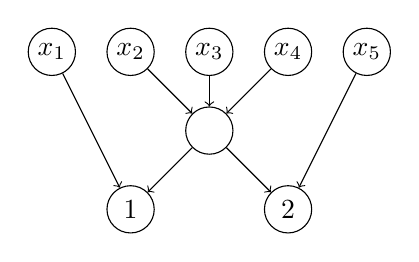
\begin{tikzpicture}
%\draw[help lines] (0,0) grid (10,6);
\foreach \x/\y/\n/\t in {0/4/x1/x_1, 1/4/x2/x_2, 2/4/x3/x_3, 3/4/x4/x_4, 4/4/x5/x_5, 2/3/a/~, 1/2/b/1, 3/2/c/2}
  \node[inner sep=0mm,circle,draw,minimum size=6mm] (\n) at (\x,\y) {$\t$};
\foreach \s/\t in {x2/a, x3/a, x4/a, a/b, x1/b, a/c, x5/c}
  \draw[->] (\s) -- (\t);
\end{tikzpicture}
\end{center}

For a~0/1-matrix~$A$, by $C(A)$ we denote the minimum
number of gates in a~circuit computing the function $Ax$.


A~{\em binary circuit} is a~circuit having no gates of fan-in more than two. It is not difficult to see that any circuit can be converted into a~binary circuit of size at most twice the size of the original circuit. For this, one just replaces every gate of fan-in~$k$, for $k>2$, by a~binary tree with $2k-2$ wires (such a~tree contains $k$~leaves hence $k-1$ inner nodes and $2k-2$ edges).

Clearly, in the binary circuit the number of gates does not exceed its size (i.e., the number of wires). And the number of gates in a~binary circuit is exactly the minimum number of semigroup operations needed to compute the corresponding function.

Note that we can view circuits as computations over some semigroup $(S,\circ)$, meaning that we can substitute instead of the variables elements of the semigroup $S$. If we fix some semigroup $(S,\circ)$ we can actually consider a circuit as a computation in the semigroups $X_S$. Moreover, we can forget about original semigroup $S$ and consider the computations in the circuit as computations in arbitrary semigroup $X$ with generators $x_1, \ldots, x_n$.


In an~important special case of the Boolean semigroup $(\{0,1\}, \lor)$, circuits we are discussing are known as {\em rectifier networks}. An overview of known lower and upper bounds for such circuits is given by Jukna in \cite[Section~13.6]{DBLP:books/daglib/0028687}.



\section{Commutative Case}\label{sec-commutative}
It is easy to see that a~matrix $A \in \{0,1\}^{n \times n}$
with~$k$ ones can be computed by a~circuit of size $O(n+k)$.
The corresponding circuit is straightforward. The main goal of
this section is to prove the same lower bound for the case
when~$A$ has~$k$ zeroes (rather than ones) and the
corresponding semigroup is commutative. The resulting circuits
are already not at all straightforward.

We prove a~sequence of more and more general result. In the first result, which is almost trivial,  commutativity is not even needed.



%\subsection{Constant Maximum Row Density}

\begin{lemma}\label{lemma:easy}
Let $X$~be {\em any} semigroup (not necessarily commutative) and let $A \in \{0,1\}^{n \times n}$ contain at most one zero in every row. Then $C(Ax) \le O(n)$.
\end{lemma}
\begin{proof}
We first precompute all prefixes and suffixes of $x_1, \dotsc, x_n$. Namely, let $p_i=x_1x_2\dotsb x_i$. All $p_i$'s can be computed in $(n-1)$ binary gates as follows:
\[p_1=x_1, p_2=p_1x_2, p_3=p_2x_3, \dotsc, p_i=p_{i-1}x_i, \dotsc, p_n=p_{n-1}x_n \, .\]
Similarly, in $(n-1)$ binary gates we compute all suffixes $s_j$
(for all $1 \le j \le n$) where $s_j=x_jx_{j+1}\dotsc x_n$. From
these prefixes and suffixes all the outputs can be computed as
follows: if a~row of~$A$ contains no zeros, the corresponding
output is~$p_n$; if a~row contains a~zero in position~$i$, the
output is $p_{i-1}s_{i+1}$ (for $i=1$ and $i=n$ we just omit
the redundant term).
\end{proof}

In the rest of the section, we assume that the underlying semigroup is commutative.
Allowing at most two zeros per row already leads to a~non-trivial
problem. We give a~sketch of its solution as
below we prove a~more general results.
It is interesting to compare the following lemma
with Corollary~\ref{cor:noncommutativetwo} that states that in
the non-commutative setting we cannot hope for linear size
circuits.

\begin{lemma} \label{lem:at_most_2}
Let $A \in \{0,1\}^{n \times n}$ contain at most two zeros in every row. Then $C(Ax) \le O(n)$.
\end{lemma}
\begin{proof}[Proof sketch]
Consider the following undirected graph: the set of nodes is $[n]$; two nodes $i$ and $j$ are joined by an edge, if there is a~row having zeros in columns~$i$ and~$j$. The graph has $n$~edges and hence it contains a cut $(L,R)$ of size at least $n/2$. This cut splits the columns of the matrix into two parts ($L$ and $R$). Let now also split the rows into two parts: the top part $T$~contains all columns that have exactly one zero in both $L$ and $R$; the bottom part $B$ contains all the remaining rows. What is nice about the top part of the matrix ($T \times (L \cup R)$) is that it can be computed by $O(n)$ gates (using Lemma~\ref{lemma:easy}). For the bottom part, let us cut all-1 columns out of it and make a recursive call. The corresponding recurrence relation is $C(n) \le an + C(n/2)$ implying $C(n)=O(n)$.
\todo[inline]{Andrey, polish this proof. Make sure that we use the same notation as in the rest of the paper. (I just copied this proof from stackexchange)}
\end{proof}

It is possible to generalize the previous lemma to the case of
any constant number of zeros in every row. Below we prove
an even more general result.

The most interesting case in the case of $X$ being free commutative semigroup.

\begin{theorem}\label{thm:main}
Suppose $S$ is a commutative semigroup. A~matrix $A \in \{0,1\}^{n \times n}$ with $k$~zeros can
be computed by a~circuit of size $O(n+k)$.
\end{theorem}

It is easy to see that the hardest case is when $X_S$ is a free commutative semigroup. Indeed, any other semigroup is the factorization of the free semigroup. Thus for any semigroup $X$ we can just use the same circuit as for free semigroups.


Thus from now on in the proof of Theorem~\ref{thm:main} we concentrate on the case of free commutative semigroup $X_S$. We build the required circuit out of the basic building blocks described below. We first show how to use these blocks and then prove their existence.

\begin{lemma}\label{lemma:decompose}
There exists a~binary~circuit of size $O(n\log n)$ such that
any range can be computed in a~single additional binary gate
using two gates of the circuit.
\end{lemma}

\begin{lemma}\label{lemma:blocks}
There exists a~binary circuit of size $O(n)$ such that any range
of length at least $\log n$ can be computed in two binary
additional gates from the gates of the circuit.
\end{lemma}

\begin{lemma}\label{lemma:permute}
Let $A \in \{0,1\}^n$ contains at most $\log n$ zeroes in
every row. Then there exists a~permutation of the rows of~$A$
such that the total length of all ranges of length
at most $\log n$ is $O(\log^4 n)$.
\end{lemma}


\begin{observation}\label{obs:transpose}
Suppose $X$ is free commutative semigroup with generators $x_1,\ldots, x_n$. Then for any $0/1$-matrix~$A$, $C(A)=C(A^T)$.
\end{observation}
\begin{proof}[Proof of Observation~\ref{obs:transpose}]
Reverse the direction of each wire in a~circuit computing~$A$ to get a~circuit computing~$A^T$.
\end{proof}



\begin{proof}[Proof of Theorem~\ref{thm:main}]
We first take a~permutation of the columns of the matrix
guaranteed by Lemma~\ref{lemma:permute}. At this stage,
we use commutativity of the ground semigroup essentially.
We will compute all the ranges of~$A$. From these ranges,
it takes $O(n+k)$ additional wires to compute all the outputs.

Denote the set of rows and the set of columns of~$A$ by~$R$
and~$C$, respectively. Let $R_0 \subseteq R$ be all the rows
having at least $\log n$ zeros and $R_1=R \setminus R_0$. We
compute the matrices $R_0 \times C$ and $R_1 \times C$
separately. In a~few words, $R_0 \times C$ is easy to compute
as it has a~small number of rows (at most $k/\log n$). $R_1 \times C$ is easy since it has a~small number of zeroes in
every row (at most $\log n$).

\emph{Computing $R_0 \times C$.} Thanks to
Observation~\ref{obs:transpose}, it suffices
to compute $C \times R_0$.
Let $|R_0|=t$. Clearly, $t \le k/\log n$.
Using Lemma~\ref{lemma:decompose}, one can compute all
ranges of $C \times R_0$ by a~circuit of size
\[O(t\log t+k)=O\left(\frac{k}{\log n} \cdot \log k+k\right)=O(k+n)\, ,\]
since $k \le n^2$.

\emph{Computing $R_1 \times C$.} Each row of
$R_1 \times C$ contains at most $\log n$ zeros. Moreover,
thanks to Lemma~\ref{lemma:permute}, the total length of all
ranges of length at most $\log n$ is $O(\log^4n)$. Hence, all
such short ranges can be computed by a~circuit of size~
$O(\log^4n)=O(n)$. It remains to compute all the ranges of
length at least~$\log n$. This can be done using Lemma~\ref{lemma:blocks}.
\end{proof}

\begin{proof}[Proof of Lemma~\ref{lemma:decompose}]
We adopt the divide-and-conquer construction by~Alon and Schieber~\cite{Alon87optimalpreprocessing}.
Split the input range $(1,n)$ into two half-ranges of
length~$n/2$:
$(1,n/2)$ and $(n/2+1,n)$.
Compute all suffixes of the left half and all prefixes of
the right half.
Using these precomputed suffixes and
prefixes one can answer any query $(l,r)$ such that $l \le n/2
\le r$ in a~single additional gate. It remains to be able to answer
queries that lie entirely in one of the halves. We do this by
constructing recursively circuits for both halves. The resulting
recurrence relation $T(n) \le 2T(n/2)+O(n)$ implies that the
resulting circuit has size at most $O(n\log n)$.
\end{proof}

\begin{proof}[Proof of Lemma~\ref{lemma:blocks}]
We use the block decomposition technique for
constructing the required circuit.
Partition the input range $(1,n)$ into $n/\log n$ ranges
of length $\log n$ and call them blocks. Compute the range
corresponding to each block (in total size $O(n)$).
%and denote
%the results by $b_1, \dotsc, b_{n/\log n}$.
Now, build a~circuit from Lemma~\ref{lemma:decompose} on
top of these blocks. The size of this circuit is $O(n)$ since the
number of blocks is $n/\log n$.

Now, compute all prefixes and all suffixes of every block. Since
the block partition the input range $(1,n)$, this also can be done
with an $O(n)$ size circuit.

Now consider any range of length at least $\log n$. Note that it
cannot lie entirely inside the block. Hence, any such range can be
decomposed into three subranges: a~suffix of a~block, a~range
of blocks, and a~prefix of a~block
(where any of the three components may be empty). For example, for $n=16$,
a~range $(2,13)$ is decomposed into a~suffix $(3,4)$ of the
first block,
a~range $(2,3)$ of blocks, and a~prefix $(13,13)$ of
the last block:
\begin{center}
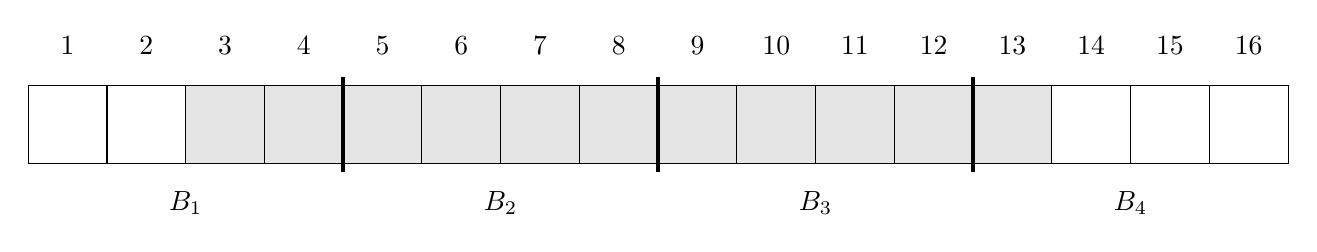
\begin{tikzpicture}
\foreach \x in {1,...,16}
  \node at (\x,2) {\x};
\draw[draw=white,fill=gray!20!white] (2.5,0.5) rectangle (13.5,1.5);
\foreach \x in {1,...,15}
  \draw (\x+0.5,0.5) -- (\x+0.5,1.5);
\draw (0.5,0.5) rectangle (16.5,1.5);
\foreach \x in {4,8,12}
  \draw[line width=.5mm] (\x+0.5,0.4) -- (\x+0.5,1.6);
\foreach \x/\i in {2/1, 6/2, 10/3, 14/4}
  \node at (\x+0.5,0) {$B_{\i}$};
\end{tikzpicture}
\end{center}
It remains to note that all these three components are already precomputed.
\end{proof}

\begin{proof}[(Probabilistic) Proof of Lemma~\ref{lemma:permute}.]
Permute the columns randomly and compute the expectation of
the total length of ranges of length at most $\log n$. Call such ranges short. Let us focus on a~single row and a~particular cell in it. Denote the number of zeros in the row by~$t$. What is the probability that it belongs to a~segment of length $\log n$? There are two cases to consider.
\begin{enumerate}
\item The cell lies close to the border, i.e., it belongs to
the first $\log n$ cells or to the last~$\log n$ cells
(the number of such cells is $2\log n$). Then,
this cell belongs to a~short range iff there is at least one zero
in $\log n$ cells close to it (on the side opposite to the border).
Hence, one zero must belong to a~set of $\log n$ cells while the remaining $t-1$ zeros may be anywhere.
The probability is then at most
\[\log n \cdot \frac{\binom{n}{t-1}}{\binom{n}{t}}=\log n \cdot \frac{t}{n-t+1}=O\left(\frac{\log^2n}{n}\right) \, .\]
\item It is not close to the border (the number of such cells is $n-2\log n$). Then, there must be a~zero on both sides of the
cell. The probability is then at most
\[\log^2 n \cdot \frac{\binom{n}{t}}{\binom{n}{t-2}}=\log^2n \cdot \frac{t(t-1)}{(n-t+1)(n-t+2)}=O\left(\frac{\log^4 n}{n^2}\right) \, .\]
\end{enumerate}
Hence, the expected total length of short ranges in one row is
\[O\left( 2\log n \cdot \frac{\log^2 n}{n} + (n-2\log n) \cdot \frac{\log^4 n}{n^2}\right)=O\left(\frac{\log^4 n}{n}\right) \, .\]
Multiplying this by the number of rows gives the desired upper bound.
\end{proof}

The construction of the circuit above is not explicit, since the proof of Lemma~\ref{lemma:permute} is randomized. We outline an explicit construction of a circuit in Appendix~\ref{subsec:constructive}.


\section{Non-commutative Case}\label{sec-non-commutative}

In the previous section, we have shown that for commutative semigroups dense linear operators can be computed by linear size circuits. A~closer look at the circuit constructions reveals that we use commutativity crucially: it is important that we may reorder the columns of the matrix. In this section, we show that this trick is unavoidable: for non-commutative semigroups, it is not possible to construct linear size circuits for dense linear operators.

%In the previous section, we have shown that for commutative semigroups dense linear operators can be computed by linear size circuits. A~closer look at the circuit constructions reveals that we use commutativity crucially: it is important that we may reorder the columns of the matrix. In this section, we show that this trick is unavoidable: for non-commutative semigroups, it is not possible to construct linear size circuits for dense linear operators. We do this by showing that, in the non-commutative case, the dense linear operator problem has linear size circuits iff the range queries problem has linear size circuits. We then use a~lower bound $\Omega(n\alpha(n))$ for the latter problem (over faithful semigroups) by Chazelle and Rosenberg~\cite{DBLP:journals/ijcga/ChazelleR91}.

\begin{theorem}\label{thm:noncommlowerbound}
For any strongly non-commutative semigroup $X$ there is a circuit to compute any dense operator of size $O(n\alpha(n))$, where $\alpha(n)$ is the inverse Ackermann function. On the other hand, there exist dense matrices~$A$ such that any circuit computing $Ax$ must have size $\Omega(n\alpha(n))$.
\end{theorem}

The upper bound follows easily by a naive algorithm: split all rows of $A$ into ranges, compute all ranges by a circuit of size $O(n\alpha(n))$ using Yao's construction~\cite{DBLP:conf/stoc/Yao82}, then combine ranges into rows of $A$ using $O(n)$ gates.

Thus we will concentrate on lower bounds. We will view the computation of the circuit as a computation in a strongly non-commutative semigroup $X$. We note that it is enough to prove the lower bound for the case of idempotent strongly non-commutative semigroups $X$. Indeed, if $X$ is not idempotent, we can factorize it by idempotency relations and obtain a strongly non-commutative idempotent semigroup $X_{id}$. A lower bound for the case of $X_{id}$ implies lower bound for the case of $X$. We provide a detailed explanation in Appendix~\ref{sec:noncommutative_extension}.

Hence, {\em until Section~\ref{sec:noncommutative_extension} we assume that $X$ is idempotent and strongly non-commutative.}

We proceed by establishing the following equivalence. We note that the equivalence between two problems is not difficult to prove for free semigroups.

\begin{theorem}\label{thm:equivalence}
For any idempotent strongly non-commutative $X$ and for any $s=\Omega(n)$ we have that commutative range queries problem has size $O(s)$ circuits iff non-commutative dense linear operator problem has size $O(s)$ circuits.
\end{theorem}

Using this theorem, it is straightforward to prove
Theorem~\ref{thm:noncommlowerbound}.

\begin{proof}[Proof of Theorem~\ref{thm:noncommlowerbound}]
By Theorem~\ref{thm:equivalence}, if non-commutative dense linear operator problem has size $s$ circuit, then the commutative range queries problem also does. However, for the latter problem it is proved by Chazelle and Rosenberg~\cite{DBLP:journals/ijcga/ChazelleR91} that $s=\Omega(n \alpha(n))$.
\end{proof}

Thus, it remains to prove Theorem~\ref{thm:equivalence}. We do this by showing the following equivalences for any $s = \Omega(n)$.

\begin{center}
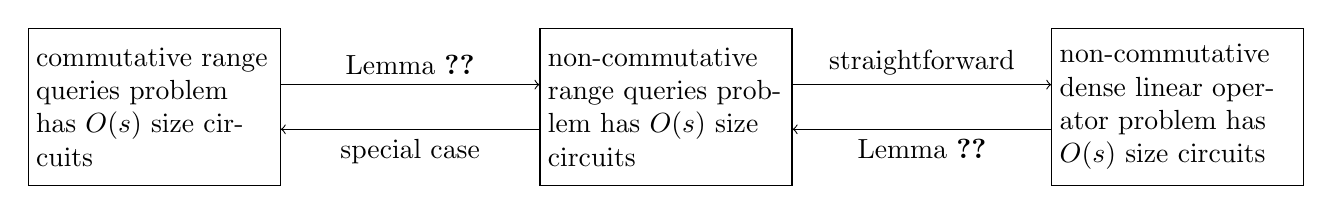
\begin{tikzpicture}
%\draw[help lines] (0,0) grid (16,6);
\tikzstyle{v}=[rectangle,draw,inner sep=1mm,text width=30mm,above right,minimum height=20mm]

\node[v] (a) at (0,0) {commutative range queries problem has $O(s)$ size circuits};

\node[v] (b) at (6.5,0) {non-commutative range queries problem has $O(s)$ size circuits};

\node[v] (c) at (13,0) {non-commutative dense linear operator problem has $O(s)$ size circuits};

\path (a.10) edge[->] node[above] {Lemma~\ref{lem:intervals}} (b.170);
\path (b.190) edge[->] node[below] {special case} (a.-10);
\path (b.10) edge[->] node[above] {straightforward} (c.170);
\path (c.190) edge[->] node[below] {Lemma~\ref{lem:dense_matrices}} (b.-10);
\end{tikzpicture}
\end{center}

In these equivalences non-commutative problems are considered over arbitrary strongly non-commutative semiring and the commutative problem is considered over free idempotent commutative semiring $X$. It is not hard to observe that if we factorize any strongly non-commutative idempotent semiring over commutativity equivalences, we obtain exactly free idempotent commutative semiring.




%To show the theorem we introduce an intermediate problem: computing non-commutative intervals by $O(n)$-size circuit.
%
%Clearly, this problem subsumes both of our problems. Indeed, if we can compute non-commutative intervals, we can compute commutative intervals by the same circuit.
%On the other hand, if we can compute non-commutative intervals, then given non-commutative dense matrix we can split it into intervals, compute them separately, then join them together in $O(n)$.
%
%Thus, it remains to show the following two lemmas.

\begin{lemma} \label{lem:dense_matrices}
If the non-commutative dense linear operator problem has size $s$ circuit then the non-commutative range queries has size $O(s)$ circuit.
%If we can compute non-commutative dense matrices by a linear size circuit, we can also compute non-commutative intervals.
\end{lemma}

\begin{lemma} \label{lem:intervals}
If the commutative version of the range queries problem has size $s$ circuits then the non-commutative version also does.
%If we can compute commutative intervals by a linear size circuit, we can also compute non-commutative intervals.
\end{lemma}

\subsection{Reducing Dense Linear Operator to Range Queries}
In this subsection, we prove Lemma~\ref{lem:dense_matrices}. Intuitively, the lemma holds as the best way to compute rows of a~dense matrix is to combine input variables in the correct order. This is shown in Lemma~\ref{lemma:correctorder}. Given this, it is easy to reduce dense linear operator problem to the range queries problem: we just ``pack'' each range query into a~separate row, i.e., for a~query $(l,r)$ we introduce a~$0/1$-row having two zeros in positions $l-1$ and $r+1$ (hence, this row consists of three queries: $(1,l-1)$, $(l,r)$, $(r+1,n)$). Then, if a~circuit computing the corresponding linear operator has a~nice property of always using the right order of variables (guaranteed by Lemma~\ref{lemma:correctorder}), one may extract the answer to the query $(l,r)$ from it.

It should be mentioned, at the same time, that idempotency is tricky. For example, it can be used to simulate commutativity: one can turn $xy$ into $yx$, by first multiplying $xy$ by~$y$ from the left and then multiplying the result by $x$ from the right (obtaining $(y(xy))x=(yx)(yx)=yx$). Using similar ideas, one can place new variables inside of already computed products. To get $xyz$ from $xz$, one multiplies it by $xyz$ first from the left and then from the right: $(xyz)xz(xyz)=xy(zxzx)yz=xy(zx)yz=xyz$.
This is not extremely impressive, since to get $xyz$ we multiply by $xyz$, but the point is that this is possible in principle.

We proceed to the formal proofs. The proof of Lemma~\ref{lem:dense_matrices} follows from the following two lemmas. A~binary circuit is called an~{\em increasing} circuit if each of its gates computes a~word that is equivalent to a~word that is a sequence of increasing variables.
Note that if a~gate in an~increasing circuit is fed by two gates~$G$ and~$H$, then the increasing sequences of variables computed by~$G$ and~$H$ are matching in a~sense that some suffix of~$G$ (possibly an empty suffix) is equal to some prefix of~$H$. Otherwise, the result is not equal to an increasing sequence of variables, due to Lemma~\ref{lem:variables_order}.

\begin{lemma}\label{lemma:correctorder}
Given a~binary circuit computing~$Ax$, one may transform it into an~increasing circuit of the same size computing the same function.
\end{lemma}

\begin{lemma}\label{lemma:matrixranges}
Given an~increasing circuit computing~$Ax$, one may transform it into a~range circuit of the same size computing all ranges of~$A$.
\end{lemma}

\begin{proof}[Proof of Lemma~\ref{lem:dense_matrices}]
Given $n$~ranges, pack them into a~matrix $A \in \{0,1\}^{n \times n}$ with at most $2n$ zeros. Take an $O(n)$ size circuit computing $Ax$ and convert it into a~binary circuit. Then, transform it into an~increasing circuit using Lemma~\ref{lemma:correctorder}. Finally, extract the answers to all the ranges from this circuit using Lemma~\ref{lemma:matrixranges}.
\end{proof}

Since the proof of Lemma~\ref{lem:dense_matrices} deals with matrices with exactly two zeros in every row, we get the following corollary that contrasts Lemma~\ref{lem:at_most_2}.
\begin{corollary}\label{cor:noncommutativetwo}
There exist matrices~$A \in \{0,1\}^{n \times n}$ with exactly two zeros in every row that requires circuits of size~$Omega(n\alpha(n))$.
\end{corollary}

\begin{proof}[Proof of Lemma~\ref{lemma:matrixranges}]
Take an~increasing circuit ${\cal C}$ computing $Ax$ and process all its gates in some topological ordering. Each gate $G$ of the original circuit computes a word equivalent to an increasing sequence of variables. We split this sequence into ranges and we put into correspondence to $G$ an ordered sequence $G_1,\ldots, G_k$ of gates of the new circuit. Each of this gates compute one of the ranges of the increasing sequence and $G \sim G_1\circ\ldots \circ G_k$.

Consider a gate $G$ of ${\cal C}$ and suppose we have already computed all gates of the new circuit corresponding to previous gates of ${\cal C}$. $G$ is the product $F \circ H$ of previous gates of ${\cal C}$. For which new range gates are already computed. Since ${\cal C}$ is increasing we have that $F$ and $H$ are matching, that is some suffix (maybe empty) of the increasing sequence computed in $F$ is equal to some prefix (maybe empty) of the increasing sequence computed in $H$ and there are no other common variables in these increasing sequences. It is easy to see that ranges for the sequence corresponding to $G$ are just the ranges for the sequences for $F$ and $H$ with possible to of them united. If needed, we compute the product of gates of the new circuit corresponding to the united ranges and the sequence of new gates for $G$ is ready

Thus, to process each gate of ${\cal C}$ we need at most one operation in the new circuit and the size of the new circuit is at most the size of ${\cal C}$.

For output gates of ${\cal C}$ we have gates in the new circuit that compute exactly ranges of output gates. Thus, in the new circuit all ranges of $A$ are computed.
\end{proof}





% to construct clauses with the correct order of variables. If this is true, then the idea is that we can extend each interval by variables on both sides (with small gaps on each side of the interval), thus obtaining a dense matrix. Then we can try to extract the computation of the intervals from the computation of the dense matrix. Since all rows of the matrix are hopefully computed by consecutively adding the variables in the correct order, we might be able to do that.



%So, we consider the free idempotent semigroup with generators $\{a_1,\ldots, a_n\}$.
%We consider the generators to be ordered from $a_1$ to $a_n$ in the increasing order. We want to compute $B \cdot \vec{a}$, where $\vec{a}=(a_1,\ldots, a_n)$ and $B$ is a boolean matrix.

%We will show that any circuit computing $B \cdot \vec{a}$ can be reconstructed into another circuit that we will call \emph{an interval circuit} without increase in the size of the circuit. In this circuit we require that each gate computes a word that is equivalent to a word consisting of increasing sequence of letters. Note that as a consequence we have that if in an interval circuit we multiply two gates $f$ and $h$, then the increasing sequences of letters computed by $f$ and $h$ are matching, that is some suffix of $f$ is equal to some suffix of $h$. Otherwise, the product is not equal to an increasing sequence of variables.

%Once we show that any circuit solving our problem can be reconstructed into an interval one, it is easy to reduce an interval problem to our problem. Note, that given a circuit computing $B \cdot \vec{a}$ for a super-dense matrix $B$ we can construct a circuit computing all intervals of this matrix. Indeed, first reconstruct a circuit into an interval one. Then, once the interval circuit is trying to multiply intervals that have gaps  between them, we just not multiply them. Later on if we try to do something with the product we have not computed we use the left of its inputs in case we try to multiply from the left, and the right input if we are multiplying from the right. So, if we need to solve an interval problem, for each interval we skip one variable on each side and add all other variables to the interval. This turn our problem into the super-dense matrix. We compute this matrix, then deduce the computation of intervals as described above.

%For each gate $g$ of the circuit we will consider the word $W_g$ computed in this gate. This word is defined recursively as a concatenation of the words corresponding to input gates. For each gate $g$ we say that the letter $a$ is \emph{good} in $W_g$ if $a$ is present in $W_g$ and $W_g$ will not be multiplied on the left by words containing larger or equal letters then $a$.

%To reconstruct a circuit into a linear one we need to introduce some notation. Consider a circuit $C$ and its gate $g$.
%We will identify gates and words that they are computing. We will treat the results of the computation of the gates as words to which gates apply concatenation operation. That is, we consider these words before we apply any equivalences in the semigroup to them.

\begin{proof}[Proof of Lemma~\ref{lemma:correctorder}]
Consider a~binary circuit~${\cal C}$ computing~$Ax$ and its gate~$G$ together with a~variable~$x_i$ it depends on.
We say that $x_i$ is \emph{good} in~$G$ if there is
a~path in~${\cal C}$ from $G$ to an output gate, on which the word is never multiplied from the left by words containing variables greater than or equal to $x_i$.
Note that if $x_i$ and $x_{i'}$ are both contained in $G$, $i<i'$, and $x_i$ is good in~$G$, then $x_{i'}$ is good in~$G$, too. That is, the set of all good variables in~$G$ is closed upwards.

Consider the largest good variable in $G$ (if there is one), denote it by $x_k$ ($x_k$ is actually just the largest variable in~$G$, unless of course there are no good variables in $G$). Let us focus on the first occurrence of $x_k$ in~$G$.

\begin{claim}
All first occurrences of other good variables in~$G$ must be to the left of the first occurrence of $x_k$.
\end{claim}

\begin{proof}
Suppose that a~good variable $x_i$ has the first occurrence to the right of (the first occurrence of) $x_k$. Consider an output gate $H$ such that there is a~path from~$G$ to~$H$ and along this path there are no multiplications of $G$ from the left by words containing variables greater than~$x_i$. Then we have $H \sim LGR$, where all variables of~$L$ are smaller then~$x_i$. Then in $H$ the variable $x_i$ appears before $x_k$ when we read from left to right, but at the same time we have that $x_k$ appears before $x_i$. This contradicts Lemma~\ref{lem:variables_order}.
\end{proof}

Now, for a~gate~$G$, define two words $\mmin_G$ and $\mmax_G$. Both these words are products of variables in the increasing order: $\mmin_G$ is the product of good letters of $G$ in the increasing order, $\mmax_G$ is the product (in the increasing order) of all letters that has first occurrences before (the first occurrence of) $x_k$. Note that $\mmin_G$ is
a~suffix of $\mmax_G$. If there are no good letters in $G$ we just let $\mmin_g=\mmax_g=\lambda$ (the empty word).
%
For the word~$W$ that has the form of the product of variables in the increasing order, we call $x_j$ a~\emph{gap variable} if it is not contained in $W$
while $W$~contains variables $x_i$ and $x_k$ with $i < j < k$.

Below we show how for a~given circuit~${\cal C}$ to construct an increasing circuit~${\cal C}'$ that for each gate~$G$ of~${\cal C}$ computes some intermediate product $P_G$ between $\mmin_G$ and $\mmax_G$: $\mmin_g$ is a~suffix of $P_G$ and $P_G$ is a~suffix of $\mmax_g$. The size of~${\cal C}'$ is at most the size of~${\cal C}$. For an output gate~$G$, $\mmin_g=\mmax_g=g$ hence the circuit ${\cal C}'$ computes the correct outputs.

To construct ${\cal C}'$, we process the gates of~${\cal C}$ in a~topological ordering. If $G$~is an input gate, everything is straightforward: in this case $\mmax_G$ is either $\lambda$ or $x_j$. Assume now that $G$ is an internal gate with predecessors~$F$ and~$H$.
Consider the set of good variables in~$G$. If there are none, we let $P_G=\lambda$. If all first occurrences of good variable of $G$ are lying in one of the predecessors ($F$~and~$H$), then they are good in the corresponding input gate. We then set $P_G$ to $P_F$ or $P_H$.

The only remaining case is that some good variables have their first occurrence in~$F$ while some others have their first occurrence in~$H$. Then the largest variable $x_k$ of~$G$ has the first occurrence in $H$ and all variables of~$F$ are smaller than~$x_k$.

\begin{claim} \label{cl: h is good}
There are no gap variables for $\mmax_H$ in~$F$.
\end{claim}

\begin{proof}
Suppose that some variable $x_i$ in~$F$ is a~gap variable for $\mmax_H$. Consider an output $C$ such that there is a path from~$G$ to~$C$ and along this path there are no multiplications of $G$ from the left by words containing variables greater than~$x_k$. Then we have $C \sim LGR$ where all variables of $L$ are smaller then~$x_k$. Consider the prefix $P$ of $C$ preceding the variable~$x_k$ and the prefix~$Q$ of $LG$ preceding the letter $x_k$.
Then by Lemma~\ref{lem:prefix_equivalence} we have $P \sim Q$. But then the variables of~$P$ and~$Q$ appear in the same order if we read the words from right to left. But this is not true (the letters in~$P$ are in the decreasing order and in~$Q$ the variable $a_i$ is not on its place), a~contradiction.
\end{proof}

\begin{claim}\label{cl: f is good}
There are no gap variables for $\mmax_F$ in~$H$.
\end{claim}

\begin{proof}
Suppose that a~variable $x_i$ in~$H$ is a~gap variable for $\mmax_F$. Consider an output~$C$ such that there is a~path from~$G$ to~$C$ and along this path there are no multiplications of~$G$ from the left by words containing variables greater than $x_l$, the largest letter of~$F$. Then we have $C \sim LGR$, where all variables of~$L$ are smaller then $x_l$. Consider the prefix~$P$ of~$C$ preceding $x_l$ and the prefix $Q$ of $LG$ preceding $x_l$.
Then by Lemma~\ref{lem:prefix_equivalence} we have $P \sim Q$. But then the variables of~$P$ and~$Q$ appear in the same order if we read the words from right to left. But this is not true (the variables in~$P$ are in the decreasing order and in~$Q$ the variable $x_i$ is not on its place), a~contradiction.
\end{proof}

We are now ready to complete the proof of Lemma~\ref{lemma:correctorder}.
Consider $P_F$ and $P_H$. By Claims~\ref{cl: h is good} and~\ref{cl: f is good}, we know that they are ranges in the same sequence of variables $\var(P_F)\cup \var(P_H)$. We know that the largest variables of $P_H$ is greater than all variables of $P_f$. Then either $P_F$ is contained in $P_H$, and then we can let $P_G=P_H$ (it contains all good variables of~$G$), or we have $P_F =PQ$ and $P_H=QR$ for some words $P, Q, R$. In this case we let $P_G = P_F \cdot P_H = PQQR=PQR$. Clearly, $\mmin_G$ is the suffix of $P_G$ and $P_G$ itself is the suffix of $\mmax_G$.
\end{proof}



\subsection{Reducing Non-commutative Range Queries to Commutative Range Queries}
%{Proof of Lemma~\ref{lem:intervals}}

In this subsection we prove Lemma~\ref{lem:intervals}.

\begin{proof}[Proof of Lemma~\ref{lem:intervals}]
We will show that any computation of commutative ranges can be reconstructed without increase in the number of gates in such a way that each gate computes a range (still commutatively; recall, that we call this a range circuit). It is easy to see that then this circuit can be reconstructed as a non-commutative circuit each gate of which computes the same range with the variables in the increasing order. Indeed, we need to make sure that each gate computes a range in such a way that all variables are in the increasing order and this is easy to do by induction. Each gate computes a product of two ranges $a$ and $b$. If one of them is contained in the other, we simplify the circuit, since the gate just computes the same range as one of its inputs (due to idempotency and commutativity). It is impossible that $a$ and $b$ are non-intersecting and have a gap between them, since then our gate does not compute a range (in a range circuit). So, if $a$ and  $b$ are non-intersecting, then they are consecutive and we just need to multiply then in the right order. If the intervals are intersecting, we just multiply then in the right order and apply idempotency.

Thus it remains to show that each commutative circuit for Range Query problem can be reconstructed into a range circuit. For this we will need some notation.

Suppose we have some circuit ${\cal C}$. For each gate $G$ denote by $\lef(G)$ the smallest index of the variable in $G$ (the leftmost variable). Analogously denote by $\righ(G)$ the largest index of the variable in $G$. Denote by $\gap(G)$ the smallest $i$ such that $x_i$ is not in $G$, but there are some $j,k$ such that $j<i<k$ and $x_j$ and $x_k$ (the smallest index of the variable that is in the gap in $G$).
%If there is no such variable (that is, $g$ computes an interval), then $\gap(g)=n+1$.
Next, fix some topological ordering of gates in ${\cal C}$ (the ordering should be proper, that is inputs to any gate should have smaller numbers). Denote by $\num(G)$ the number of a gate in this ordering. Finally, by $\out(G)$ denote the out-degree of $G$.

For each gate that computes a non-range consider the tuple
$$
\tup(G)=(\lef(G),\gap(G),\num(G),-\out(G)).
$$ For the circuit ${\cal C}$ consider $\tup({\cal C}) = \min_G \tup(G)$, where the minimum is considered in the lexicographic order and is taken over all non-range gates. If there are no non-range gates we let $\tup({\cal C})=\infty$. This is our semi-invariant, we will show that if we have a circuits that is not a range circuit, we can reconstruct it to increase  its $\tup$ (in the lexicographic order) without increasing its size. Since $\tup$ ranges over a finite set, we can reconstruct the circuit repeatedly and end up with a range circuit.

Now we are ready to describe a reconstruction of a circuit. Consider a circuit ${\cal C}$ that is not a range circuit. And consider a gate $G$ such that $\tup(G)=\tup({\cal C})$ (it is clearly unique). Denote by $A$ and $B$ two inputs of $G$. Let $i=\lef(G)$ and $j=\gap(G)$, that is $x_i$ is the variable with the smallest index in $G$ and $x_j$ is the first gap variable of $G$ (it is not contained in $G$).

The variable $x_i$ is contained in at least one of $A$ and $B$. Consider the gate among $A$ and $B$ that contains $x_i$. It also contain all variables between $x_i$ and $x_j$ (but not $x_j$), since the converse would contradict minimality of $G$ (by the second coordinate of $\tup$). But this gate cannot have $x_j$ as a gap variable: it would also contradict minimality of $G$ (by the third coordinate of $\gap$). Thus this gate is exactly the interval $[x_i,x_j)$ (by this we denote the product of variables from $x_i$ to $x_j$ excluding $x_j$). In particular, only one of $A$ and $B$ contains $x_i$: otherwise they are both $[x_i,x_j)$ and $x_j$ is not a gap variable for $G$.

From now on we assume that $A$ contains $x_i$, that is $A=[x_i,x_j)$.
%Note that then $b$ contains all variables to the right of $x_j$, in particular the variable with the largest index in $g$.

Now we consider all gates $H_1,\ldots, H_k$ that have edges leading from $G$. Denote by $F_1,\ldots, F_k$ their other inputs. If $k$ is equal to $0$, we can remove $G$ and reduce the circuit. Now we consider cases.

\emph{Case 1.} Suppose that there is $l$ such that $\lef(F_l) \leq \lef(G)$. Then $F_l$ contains all variables in $[x_i,x_j)$ (the contrapositive contradicts the minimality of $g$ by the second coordinate of $\gap$). Thus $F_l$ contains $A$. Then, we can restructure the circuit by feeding $B$ to $H_l$ instead of $G$. This does not change the value of the gate computed by $H_l$ and reduces $\out(G)$. Thus $\tup({\cal C})$ increases and we are done.

\emph{Case 2.} Suppose that for all $l$ we have $\lef(F_l)>\lef(G)$. Consider $l$ such that $F_l$ has the minimal $\righ(F_l)$ (if there are several such $l$ pick among them the one with the minimal $\num(F_l)$). Now we restructure the circuit in the following way. We feed $F_l$ to $G$ instead of $A$. We feed $A$ to $H_l$ instead of $F_l$. We feed $H_l$ to all other $H_p$'s instead of $G$. It is not hard to see that all these reconstructions are valid, that is, do not create cycles (there were no paths from $G$ to $F_l$ since $\lef(G)<\lef(F_l)$; there was a path from $A$ to $H_l$, so there was no path in the reversed direction; there was no path from $H_p$ to $G$, $A$ and $F_l$ due to the minimality property of $F_l$, so there is no path from $H_p$ to $H_l$). Note that they might require reordering of the circuit gates, since we create edges between previously incomparable $H$-gates and between $F_l$ and $G$. But the reording changes only for the gates with $\num$ greater than $\num(G)$ and may only reduce $\num(F_l)$ to be smaller than $\num(G)$. But this can only increase $\tup(G)$ and since $\lef(F_l)>\lef(G)$ this can only increase $\tup({\cal C})$.

Observe, that the circuit still computes the outputs correctly. The changes are in the gates $H_1\ldots, H_k$ (and also in $G$, but $H_1,\ldots, H_k$ are all of its outputs). $H_l$ does not change. Other $H_p$'s might have changed, they now additionally include variables of $F_l$. But note that all of these variables are in between of $\lef(H_p)$ and $\righ(H_p)$, so they must be presented in the output gates connected to $H_p$ anyway.

Now, observe that $\tup(G)$ has increased (by the first coordinate). There are no new gates with smaller $\lef$. Among gates with the minimal $\lef$ there are no new gates with smaller $\gap$. Among gates with minimal $(\lef,\gap)$ all gates have larger $\num$ then $G$. Thus $\tup({\cal C})$ increased and we are done.
\end{proof}


% TODO: Uncomment in the final version.
% \section*{Acknowledgments}
% We thank Paweł Gawrychowski for pointing us out to the paper~\cite{DBLP:journals/ijcga/ChazelleR91}.

\bibliographystyle{plain}
\bibliography{text}

\section{Appendix}
\input range_queries_applications
\input approaches
\input constructive

\subsection{General Non-commutative Case}\label{sec:noncommutative_extension}

In this section we provide a detailed explanation of the reduction in Theorem~\ref{thm:noncommlowerbound} from general semigroups to idempotent semigroup.

Consider arbitrary strongly non-commutative semigroup $X$. Consider a new semigroup $X_{id}$ over the same set of generators that is a factorization of $X$ by idempotency relations $W^2\sim W$ for all words $W$ in the alphabet $\{x_1,\ldots, x_n\}$.

\begin{lemma} \label{lem:idempotisation}
If $X$ is strongly non-commutative, then $X_{id}$ is also strongly non-commutative.
\end{lemma}

\begin{proof}
Suppose $W$ and $W'$ are words in the alphabet $\{x_1,\ldots, x_n\}$ and $W \sim W'$ in $X_{id}$. This means that there is a sequence $W_0,\ldots, W_k$ of words in the same alphabet such that $W=W_0$, $W'=W_k$ and for each $i$ either $W_i \sim W_{i+1}$ in $X$, or $W_{i+1}$ is obtained from $W_i$ by one application of the idempotency equivalence to some subword of $W_i$. Clearly, it is enough to check that the conditions of Definition~\ref{def:strong_non_commutativity} are satisfied in $X_{id}$ for each consecutive pair $W_i$ and $W_{i+1}$.

If $W_i \sim W_{i+1}$ in $X$, then the conditions of Definition~\ref{def:strong_non_commutativity} follows from the strong non-commutativity of $X$.

Suppose now that $W_{i+1}$ is obtained from $W_{i}$ by substituting some subword $A$ by $A^2$ (the symmetrical case is analyzed in the same way). We will show that initial marks of $W_i$ and $W_{i+1}$ are the same and $U_{i} \sim U_{i+1}$ in $X_{id}$, where $U_{i}$ and $U_{i+1}$ are initials of $W_i$ and $W_{i+1}$ respectively. For the terminals and terminal marks the proof is completely analogous.

Suppose $A$ lies to the left of initial mark in $W_i$ and we substitute $A$ by $A^2$. Then the initial mark is unaltered and in the initial $U_i$ we also substitute $A$ by $A^2$. Thus in this case $U_{i+1}$ is obtained from $U_i$ by idempotency relation.

Suppose $A$ contains initial mark of $W_i$ or lies to the right of it. Then after the substitution of $A$ by $A^2$ the initial mark is still the same and the initial $U_i$ also does not change.
\end{proof}

Now we outline the reduction of the lower bound in Theorem~\ref{thm:noncommlowerbound} from idempotent semigroup to the general case..

Suppose $X$ is strongly non-commutative and suppose that for $X$ all dense operators can be computed by circuits of size at most $s$.

Consider a semigroup $X_{id}$ as introduced above. By Lemma~\ref{lem:idempotisation} $X_{id}$ is also strongly non-commutative. On the other hand, since $X_{id}$ is a factorization of $X$ any circuit computing dense operator over $X$ also computes the same dense operator over $X_{id}$. Thus, by other assumption there are circuits of size at most $s$ for all dense operators over $X_{id}$. Finally, $X_{id}$ is idempotent, so by the special case of our theorem we have $s = \Omega(n \alpha(n))$ and we are done.



\end{document}